%\documentclass[9pt]{scrartcl}
\documentclass[a4paper]{article}
\usepackage[]{amsmath}
\usepackage{tikz}
\usetikzlibrary{positioning}
%\usepackage{helvet}
\usepackage{listings}
\usepackage{geometry}
%\geometry{textheight=\paperheight, noheadfoot, nomarginpar}
\usetikzlibrary{positioning,shapes,shadows}
\renewcommand{\familydefault}{\sfdefault}

\tikzstyle{abstract}=[rectangle, draw=black, fill=gray!20, text centered,  text=black, text width=12.5mm]
\tikzstyle{spacestyle}=[rectangle, draw=black, fill=gray!20, text centered,  text=black, text width=50mm]

\lstset{
        language=python,
        basicstyle=\fontencoding{T1}\ttfamily,
        commentstyle=\color{gray},
        keywordstyle=\color{OliveGreen},
        frame=single,
        backgroundcolor=\color{lightlightgray},
        tabsize=2,
        %deletestring=[d]",
        %escapechar=\%,
        numbers=left,
        showstringspaces=false,
}
\usepackage[explicit]{titlesec} 
\titleformat{\section}{\normalfont\Large\bfseries}{}{0em}{#1}
\titleformat{\subsection}{\normalfont\bfseries}{}{0em}{--#1}

\newcommand{\mykey}[2]{%
\begin{tikzpicture} \node (Item) [abstract, minimum size=12.5mm, align=center]
{\vrule height 12pt depth 8pt width 0pt\textbf{#1} \\\vrule height 6pt depth 8pt width 0pt\parbox{1.25cm}{\centering{\fontsize{6pt}{8pt}\selectfont{#2}}}};%
\end{tikzpicture}}


\begin{document}
\begin{center}
\Large{Diagram}
\end{center}
\noindent%


\section {Vector clock diagram}
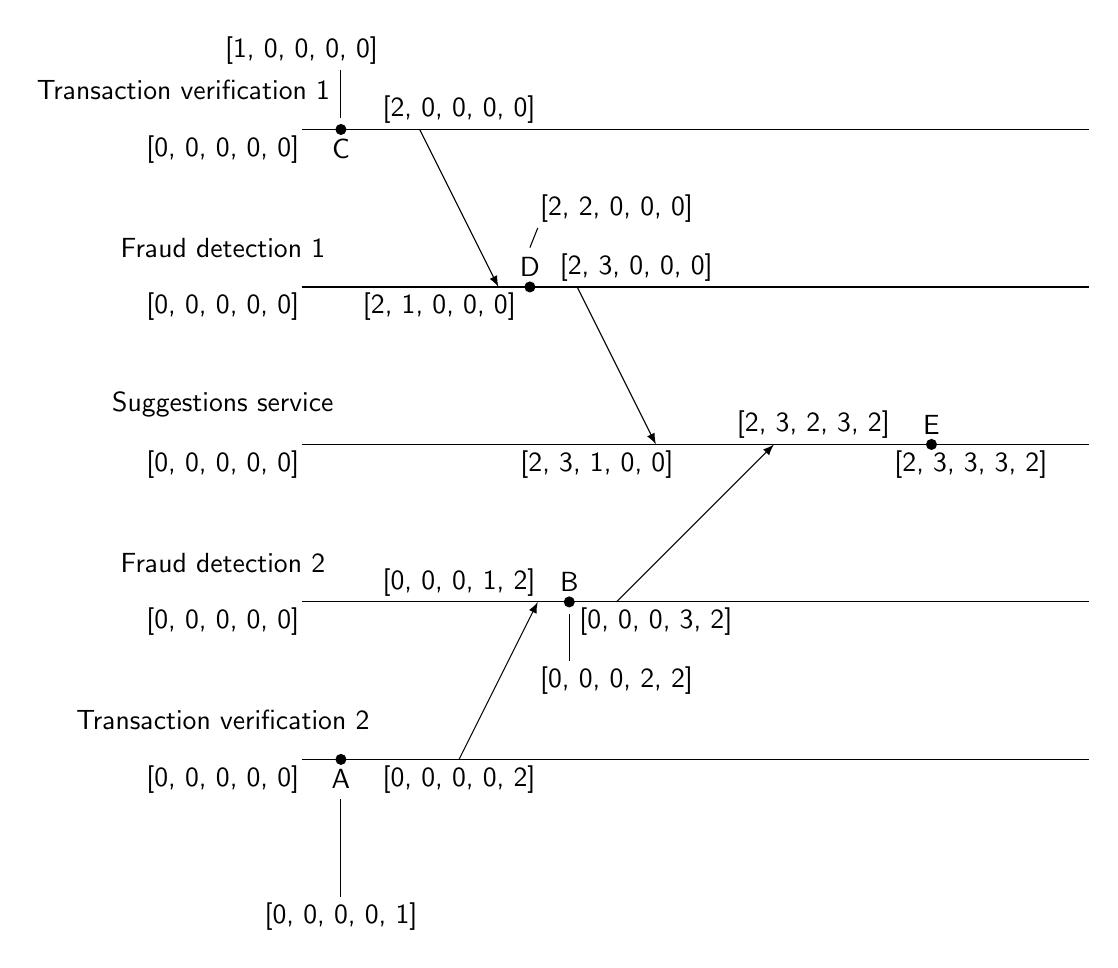
\begin{tikzpicture}

\node at (0, 0.5) {Transaction verification 2};
\node at (0, -0.25) {[0, 0, 0, 0, 0]};
\node at (0, 2.5) {Fraud detection 2};
\node at (0, 1.75) {[0, 0, 0, 0, 0]};
\node at (0, 4.5) {Suggestions service};
\node at (0, 3.75) {[0, 0, 0, 0, 0]};
\node at (0, 6.5) {Fraud detection 1};
\node at (0, 5.75) {[0, 0, 0, 0, 0]};
\node at (-0.5, 8.5) {Transaction verification 1};
\node at (0, 7.75) {[0, 0, 0, 0, 0]};

% Draw horizontal lines
\draw (1,0) -- (11,0);
\draw (1,2) -- (11,2);
\draw (1,4) -- (11,4);
\draw (1,6) -- (11,6);
\draw (1,8) -- (11,8);

\node at (3, -0.25) {[0, 0, 0, 0, 2]};
\draw[-latex] (3, 0) -- (4, 2);
\node at (3, 2.25) {[0, 0, 0, 1, 2]};
\node at (5.5, 1.75) {[0, 0, 0, 3, 2]};
\draw[-latex] (5, 2) -- (7, 4);

\node at (3, 8.25) {[2, 0, 0, 0, 0]};
\draw[-latex] (2.5, 8) -- (3.5, 6);
\node at (2.75, 5.75) {[2, 1, 0, 0, 0]};
\node at (5.25, 6.25) {[2, 3, 0, 0, 0]};
\draw[-latex] (4.5, 6) -- (5.5, 4);
\node at (4.75, 3.75) {[2, 3, 1, 0, 0]};

\node at (7.5, 4.25) {[2, 3, 2, 3, 2]};

\fill (1.5,0) circle [radius=2pt];
\node at (1.5,-0.25) {A};

\fill (4.4,2) circle [radius=2pt];
\node at (4.4,2.25) {B};

\fill (1.5,8) circle [radius=2pt];
\node at (1.5,7.75) {C};

\fill (3.9,6) circle [radius=2pt];
\node at (3.9,6.25) {D};

\fill (9,4) circle [radius=2pt];
\node at (9,4.25) {E};


\node at (1.5, -2) {[0, 0, 0, 0, 1]};
\draw (1.5, -1.75) -- (1.5, -0.5);

\node at (5, 1) {[0, 0, 0, 2, 2]};
\draw (4.4, 1.25) -- (4.4, 1.85);

\node at (1, 9) {[1, 0, 0, 0, 0]};
\draw (1.5, 8.75) -- (1.5, 8.15);

\node at (5, 7) {[2, 2, 0, 0, 0]};
\draw (3.9, 6.5) -- (4, 6.75);

\node at (9.5, 3.75) {[2, 3, 3, 3, 2]};


\end{tikzpicture}


\end{document}